\epigraph{\textit{'A helicopter does not want to fly, it just vibrates so much that the ground rejects it.'}}{Kurt Vonnegut}

\section{Optimal control of pitch/travel and elevation with and without feedback (10.4)}

%%%%%%%%%%%%%%%%%%%%%%%%%%%%%%%%%%%%%%%%%%%%%%%%%%%%%%%%%%%%
\subsection{Discretisation with elevation states (10.4.1)} \label{10.4.1}
%%%%%%%%%%%%%%%%%%%%%%%%%%%%%%%%%%%%%%%%%%%%%%%%%%%%%%%%%%%%
We will re-formulate the continuous system \eqref{eq:system} with additional states for elevation $e$ and elevation rate $\dot{e}$. The system with new state and input vectors \eqref{eq:state_input} and state equations \eqref{eq:state_eqns} is expressed by the matrices shown in \eqref{eq:matrices}.

\begin{equation}\label{eq:system}
	\V{\dot{x}}	= \M{A} \V{x} + \M{B} \V{u}
\end{equation}

\begin{equation}\label{eq:state_input}
	\V{x} =
	\begin{bmatrix}
		\lambda & r & p & \dot{p} & e & \dot{e}
	\end{bmatrix}\transpose
	,\qquad
	\V{u} =
	\begin{bmatrix}
		p_{c} & e_{c}
	\end{bmatrix}\transpose
\end{equation}

\begin{equation}\label{eq:state_eqns}
\begin{aligned}
	\dot{\lambda}	&= r \\
	\dot{r} 		&= - K_{2} p \\
	\dot{p}			&= \dot{p} \\
	\ddot{p}		&= K_{1} K_{pp} (p_{c} - p) - K_{1} K_{pd} \dot{p} \\
	\dot{e}			&= \dot{e} \\
	\ddot{e}		&= K_{3} K_{ep} (e_{c} - e) - K_{3} K_{ed} \dot{e}
\end{aligned}
\end{equation}

\begin{equation}\label{eq:matrices}
	\V{\dot{x}} =
	\underbrace{
		\begin{bmatrix}
			0 & 1 & 0				& 0				& 0				& 0				\\
			0 & 0 & -K_{2}			& 0				& 0				& 0				\\
			0 & 0 & 0				& 1				& 0				& 0				\\
			0 & 0 & -K_{1}K_{pp}	& -K_{1}K_{pd}	& 0				& 0				\\
			0 & 0 & 0				& 0 			& 0				& 1				\\
			0 & 0 & 0				& 0				& -K_{3}K_{ep}	& -K_{3}K_{ed}	\\
		\end{bmatrix}
	}_{\M{A}_{c}}
	\V{x} +
	\underbrace{
		\begin{bmatrix}
			0			& 0				\\
			0			& 0				\\
			0			& 0				\\
			K_{1}K_{pp}	& 0				\\
			0			& 0				\\
			0			& K_{3}K_{ep}	\\
		\end{bmatrix}
	}_{\M{B}_{c}}
	\V{u}
\end{equation}

%%%%%%%%%%%%%%%%%%%%%%%%%%%%%%%%%%%%%%%%%%%%%%%%%%%%%%%%%%%%
\subsection{Discretisation again (10.4.2)}
%%%%%%%%%%%%%%%%%%%%%%%%%%%%%%%%%%%%%%%%%%%%%%%%%%%%%%%%%%%%
As in Section \ref{sec:disc1}, we again need to discretize the system. The procedure is the same; refer to the earlier Section for clarification. The result can be seen in \eqref{eq:matrix_4.2_A} and \eqref{eq:matrix_4.2_B}.

\begin{equation}
\begin{aligned}
	\V{x}_{k+1}	&= \V{x}_{k} + \left( \M{A}_{c} \V{x}_{k} + \M{B}_{c} \V{u}_{k} \right) h \\
				&= \underbrace{\left( \Mc{I} + h \M{A}_{c} \right)}_{\M{A}} \V{x}_{k}
				+ \underbrace{h \M{B}_{c}}_{\M{B}} \V{u}_{k} \\
\end{aligned}
\end{equation}

\begin{equation}\label{eq:matrix_4.2_A}
	\M{A} =
	\begin{bmatrix}
		1 & h & 0				& 0					& 0				& 0					\\
		0 & 1 & -hK_{2}			& 0					& 0				& 0					\\
		0 & 0 & 1				& h					& 0				& 0					\\
		0 & 0 & -hK_{1}K_{pp}	& 1-hK_{1}K_{pd}	& 0				& 0					\\
		0 & 0 & 0				& 0					& 1				& h					\\
		0 & 0 & 0				& 0					& -hK_{3}K_{ep}	& 1-hK_{3}K_{ed}	\\
	\end{bmatrix}
\end{equation}

\begin{equation}\label{eq:matrix_4.2_B}
	\M{B} =
	\begin{bmatrix}
		0				& 0				\\
		0				& 0				\\
		0				& 0				\\
		hK_{1}K_{pp}	& 0				\\
		0				& 0				\\
		0				& hK_{3}K_{ep}	\\
	\end{bmatrix}
\end{equation}

%%%%%%%%%%%%%%%%%%%%%%%%%%%%%%%%%%%%%%%%%%%%%%%%%%%%%%%%%%%%
\subsection{Solution of the optimization problem (10.4.3)}
%%%%%%%%%%%%%%%%%%%%%%%%%%%%%%%%%%%%%%%%%%%%%%%%%%%%%%%%%%%%

The cost function is now extended to include the elevation state, which gives us \eqref{eq:cost_function_w_elev}, with constrains given by \eqref{eq:cost_constraint_w_elev}. 

\begin{equation} \label {eq:cost_function_w_elev}
	\phi = \sum\limits_{i=1}^N (\lambda_i - \lambda_f)^2 + q_1 p_{ci}^2 + q2 e_{ci}^2
\end{equation}

\begin{equation} \label{eq:cost_constraint_w_elev}
	\alpha \exp (-\beta (\lambda_k - \lambda_t)^2) -e_k \leq 0, \quad k \in \{ 1, ..., N \}
\end{equation}

In \eqref{eq:cost_constraint_w_elev}, we used the values $\alpha = 0.2$, $\beta = 20$ and $\lambda_t = \frac{2 \pi}{3}$.
We use \texttt{fmincon} to get the result of the cost function with the constraints. The parameters used are  \texttt{vlb} and \texttt{vub}, which are vectors containing the linear constraints; \texttt{mycon}, which returns the nonlinear constraints; and \texttt{Aeq} and \texttt{beq} which are the matrices for the problem to be solved. We also send in the cost function itself and the initial values \texttt{z0}.
\begin{lstlisting}
costf = @(z) 0.5*z'*Q*z;
z = fmincon(costf, z0, [], [], Aeq, beq, vlb, vub, @mycon);
\end{lstlisting}

%%%%%%%%%%%%%%%%%%%%%%%%%%%%%%%%%%%%%%%%%%%%%%%%%%%%%%%%%%%%
\subsection{Comparison of performance with and without feedback(10.4.4)}
%%%%%%%%%%%%%%%%%%%%%%%%%%%%%%%%%%%%%%%%%%%%%%%%%%%%%%%%%%%%
Without feedback the pitch goes to 0 when $\lambda = \lambda_f$, but does not compensate to avoid overshoot. With feedback, the helicopter will change its pitch to the opposite direction, making the helicopter stop and stay still at $\lambda = \lambda_f$. 

\begin{figure}[H]
	\centering
	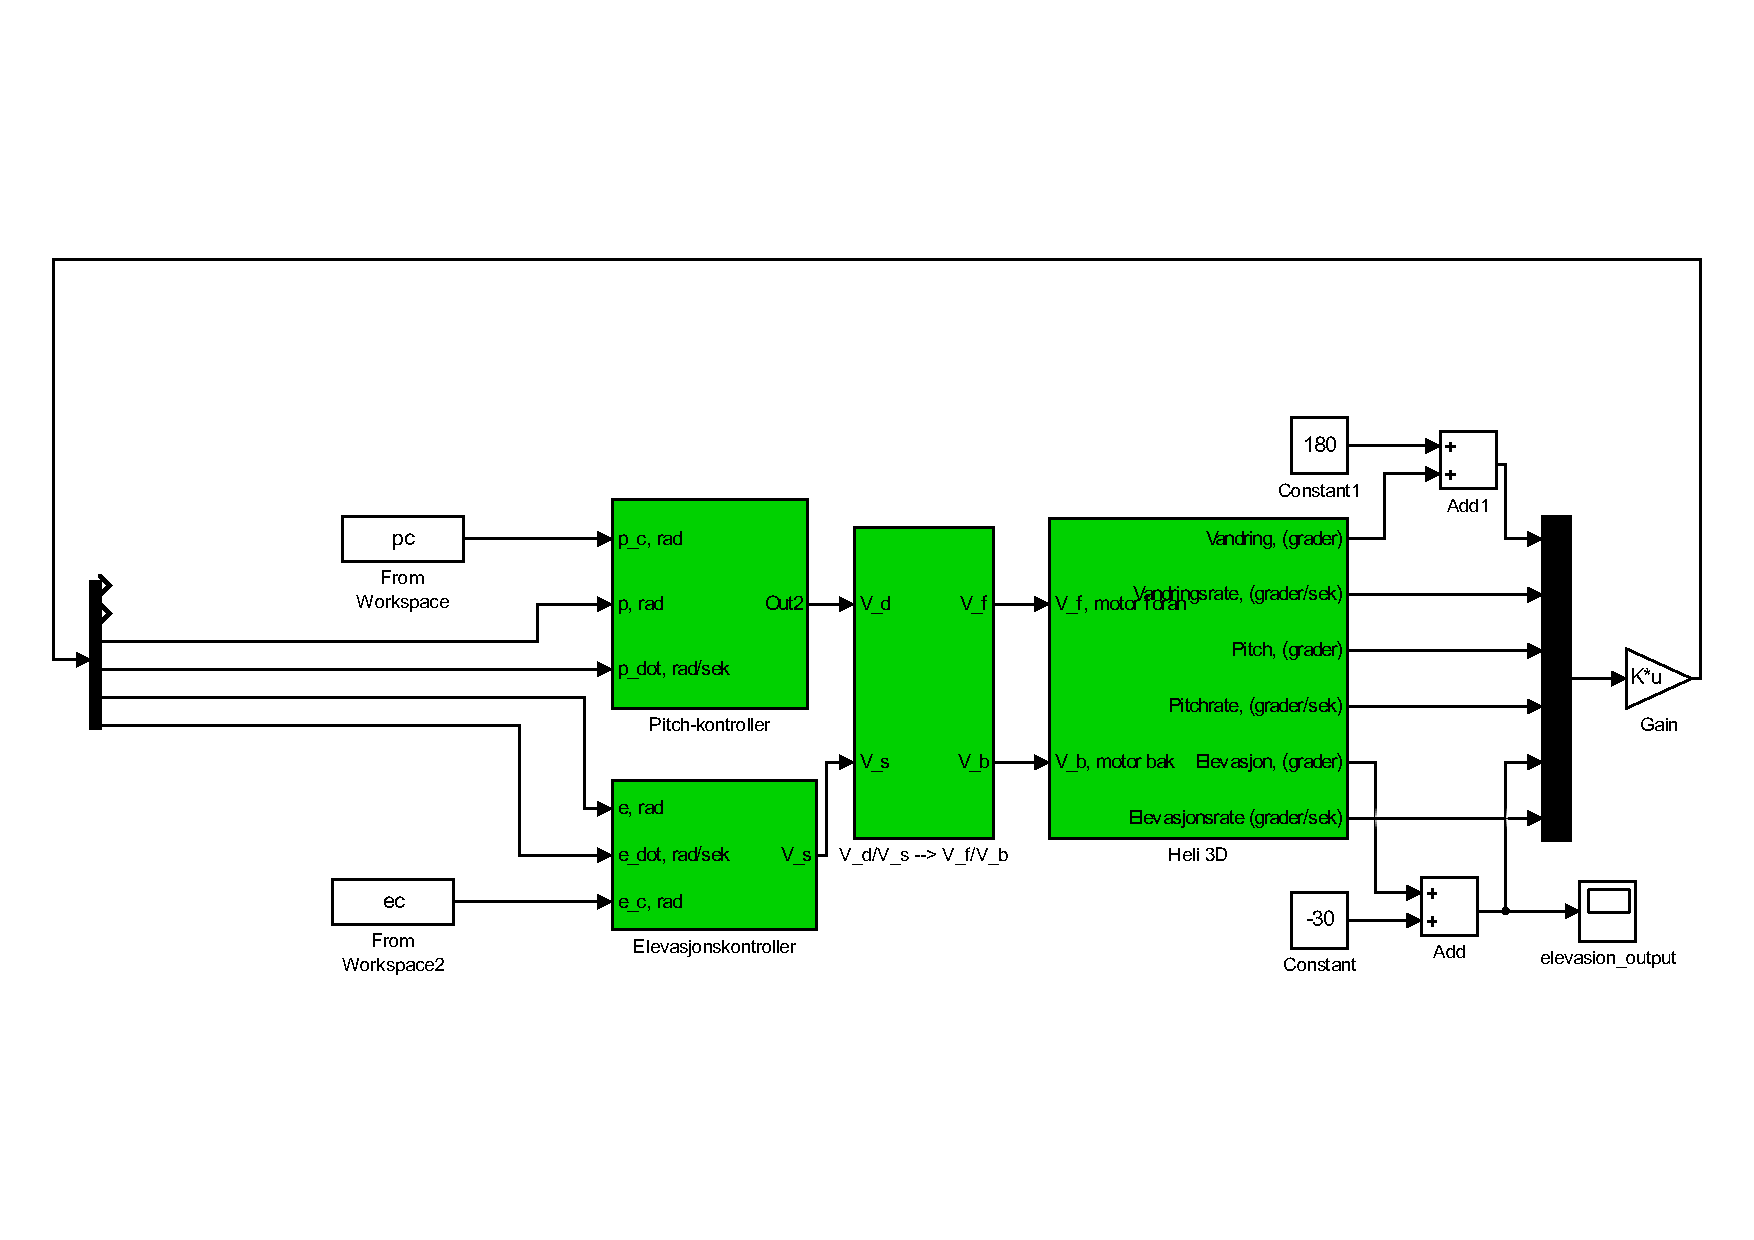
\includegraphics[width=\textwidth, trim=2cm 5cm 2cm 2cm]{simulinkmodels/heldag4UnFeed}
	\caption{Simulink model of the system without feedback}
	\label{fig:heldag4UnFeed}
\end{figure}

\begin{figure}[H]
	\centering
	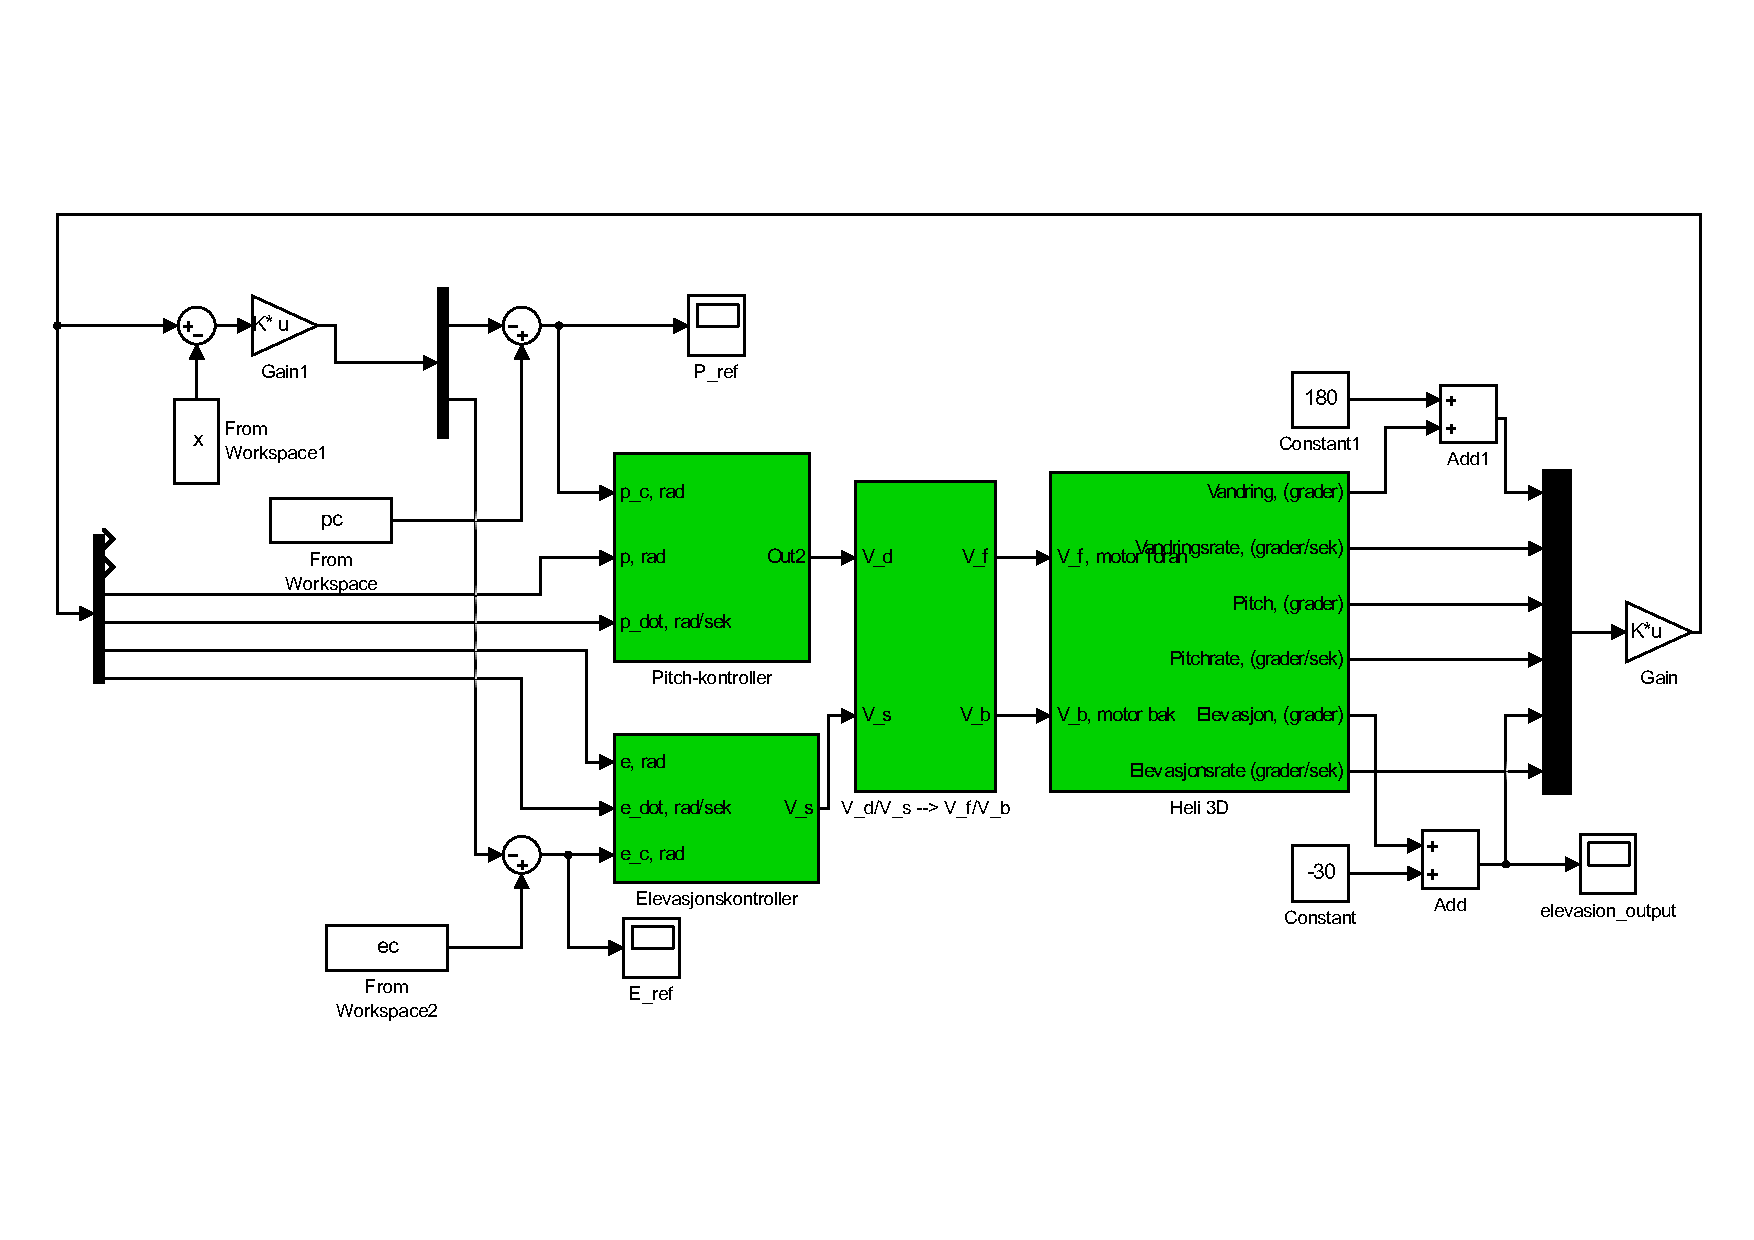
\includegraphics[width=\textwidth, trim=2cm 5cm 2cm 2cm]{simulinkmodels/heldag4medFeed}
	\caption{Simulink model of the system with feedback}
	\label{fig:heldag4medFeed}
\end{figure}

\begin{figure}[H]
	\centering
	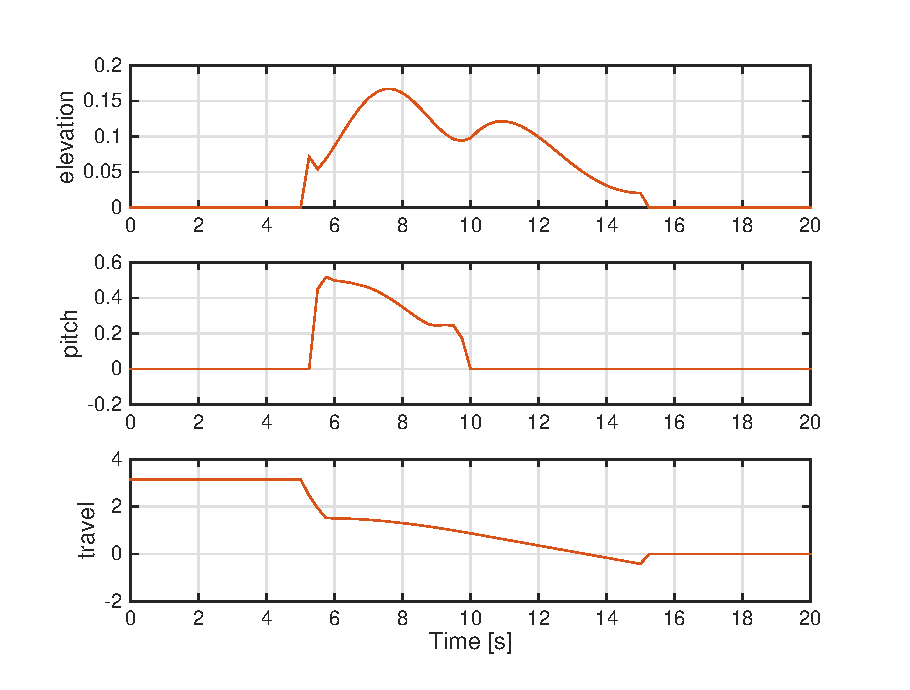
\includegraphics[width=\textwidth]{day4_calc_outputs}
	\caption{Optimal path}
	\label{fig:estimatedDay201}
\end{figure}

\begin{figure}[H]
	\centering
	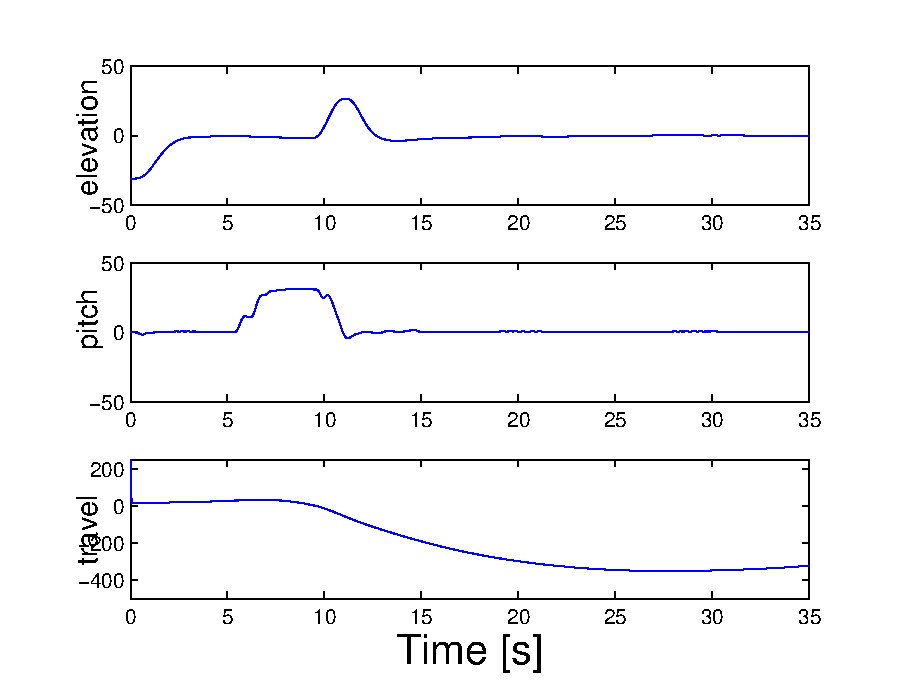
\includegraphics[width=\textwidth]{day4_nofeed}
	\caption{Running the helicopter without feedback}
	\label{fig:day4nofeed}
\end{figure}


\begin{figure}[H]
	\centering
	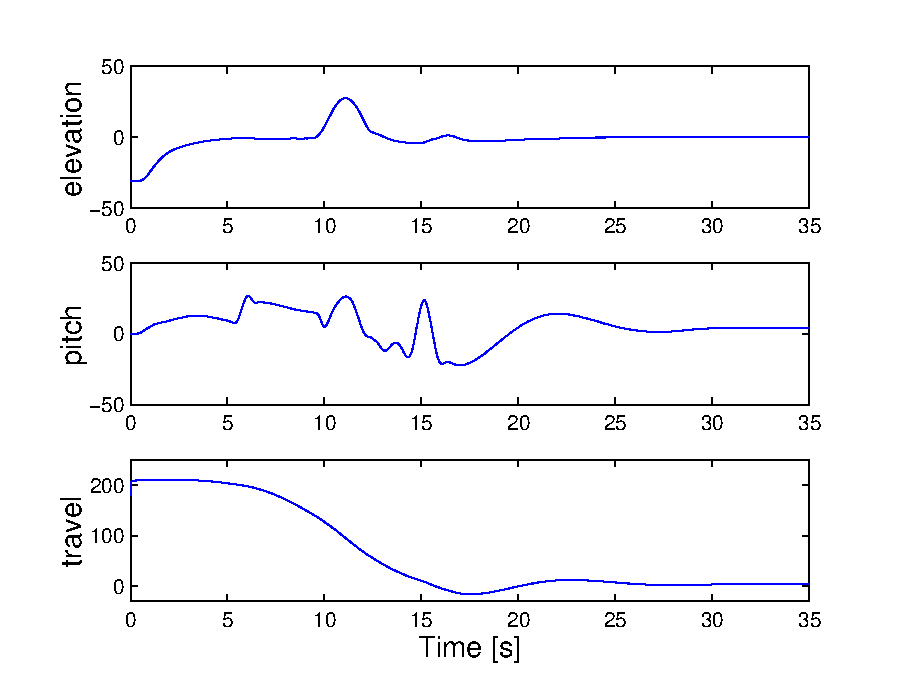
\includegraphics[width=\textwidth]{day4_yesfeed}
	\caption{Running the helicopter with feedback}
	\label{fig:day4yesfeed}
\end{figure}

As we can see in the sensor data from the model without feedback, the helicopter does not stop at $\lambda = \lambda_f$, but keeps moving. In the model with feedback, however, it does stop at $\lambda = \lambda_f$, but the change in pitch to keep it still in the reference point also makes the helicopter elevate a bit, as can be seen in the plot at roughly 16 seconds. It also overshoots slightly, but converges at the setpoint.

In the calculated outputs you can see that it also expects some change in the pitch when trying to stop at the reference point, but it is much more subtle than the real behaviour, especially with feedback. This would correspond better if the LQR was tuned better (how the LQR was tuned can be seen in the code in the appendix). In the measured values of the model without feedback, this is more similar to the calculated pitch, but the travel is a bit off, as the helicopter keeps gliding after it reaches the reference point. This is improved in the model with feedback, although it does not stop as quickly and smoothly as the calculated output would suggest.

%%%%%%%%%%%%%%%%%%%%%%%%%%%%%%%%%%%%%%%%%%%%%%%%%%%%%%%%%%%%
\subsection{Discussion of decoupled states (10.4.5)}
%%%%%%%%%%%%%%%%%%%%%%%%%%%%%%%%%%%%%%%%%%%%%%%%%%%%%%%%%%%%
In our model the elevation and the elevation rate are completely decoupled from the other states, which isn't really realistic. In real life the pitch and pitch rate of the helicopter would have an effect on both the elevation rate and the elevation itself. This will result in an offset from the calculated optimal trajectory.  
By modelling the system with the elevation and travel coupled with the pitch, you will remove the offset at the cost of a more complex model.